
\documentclass[border={0pt 0pt 0pt 0pt}]{standalone}
\usepackage{tikz-cd,tikz-3dplot} 
\usetikzlibrary{calc,intersections,through,backgrounds,decorations.pathmorphing, decorations.shapes,decorations.markings,patterns}
%include other needed packages here   
\begin{document}
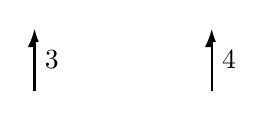
\begin{tikzpicture}[scale=3]
\foreach \y/\ytext in {-0.5/3,0.25/4}
\draw[-{Latex[]},thick] (\y cm,-0.3cm) to node[anchor=west,fill=white] {$\ytext$} (\y cm,-1pt);
\end{tikzpicture}
\end{document}